\chapter{Az új módszer}
%\begin{figure}[H]
%\begin{center}
%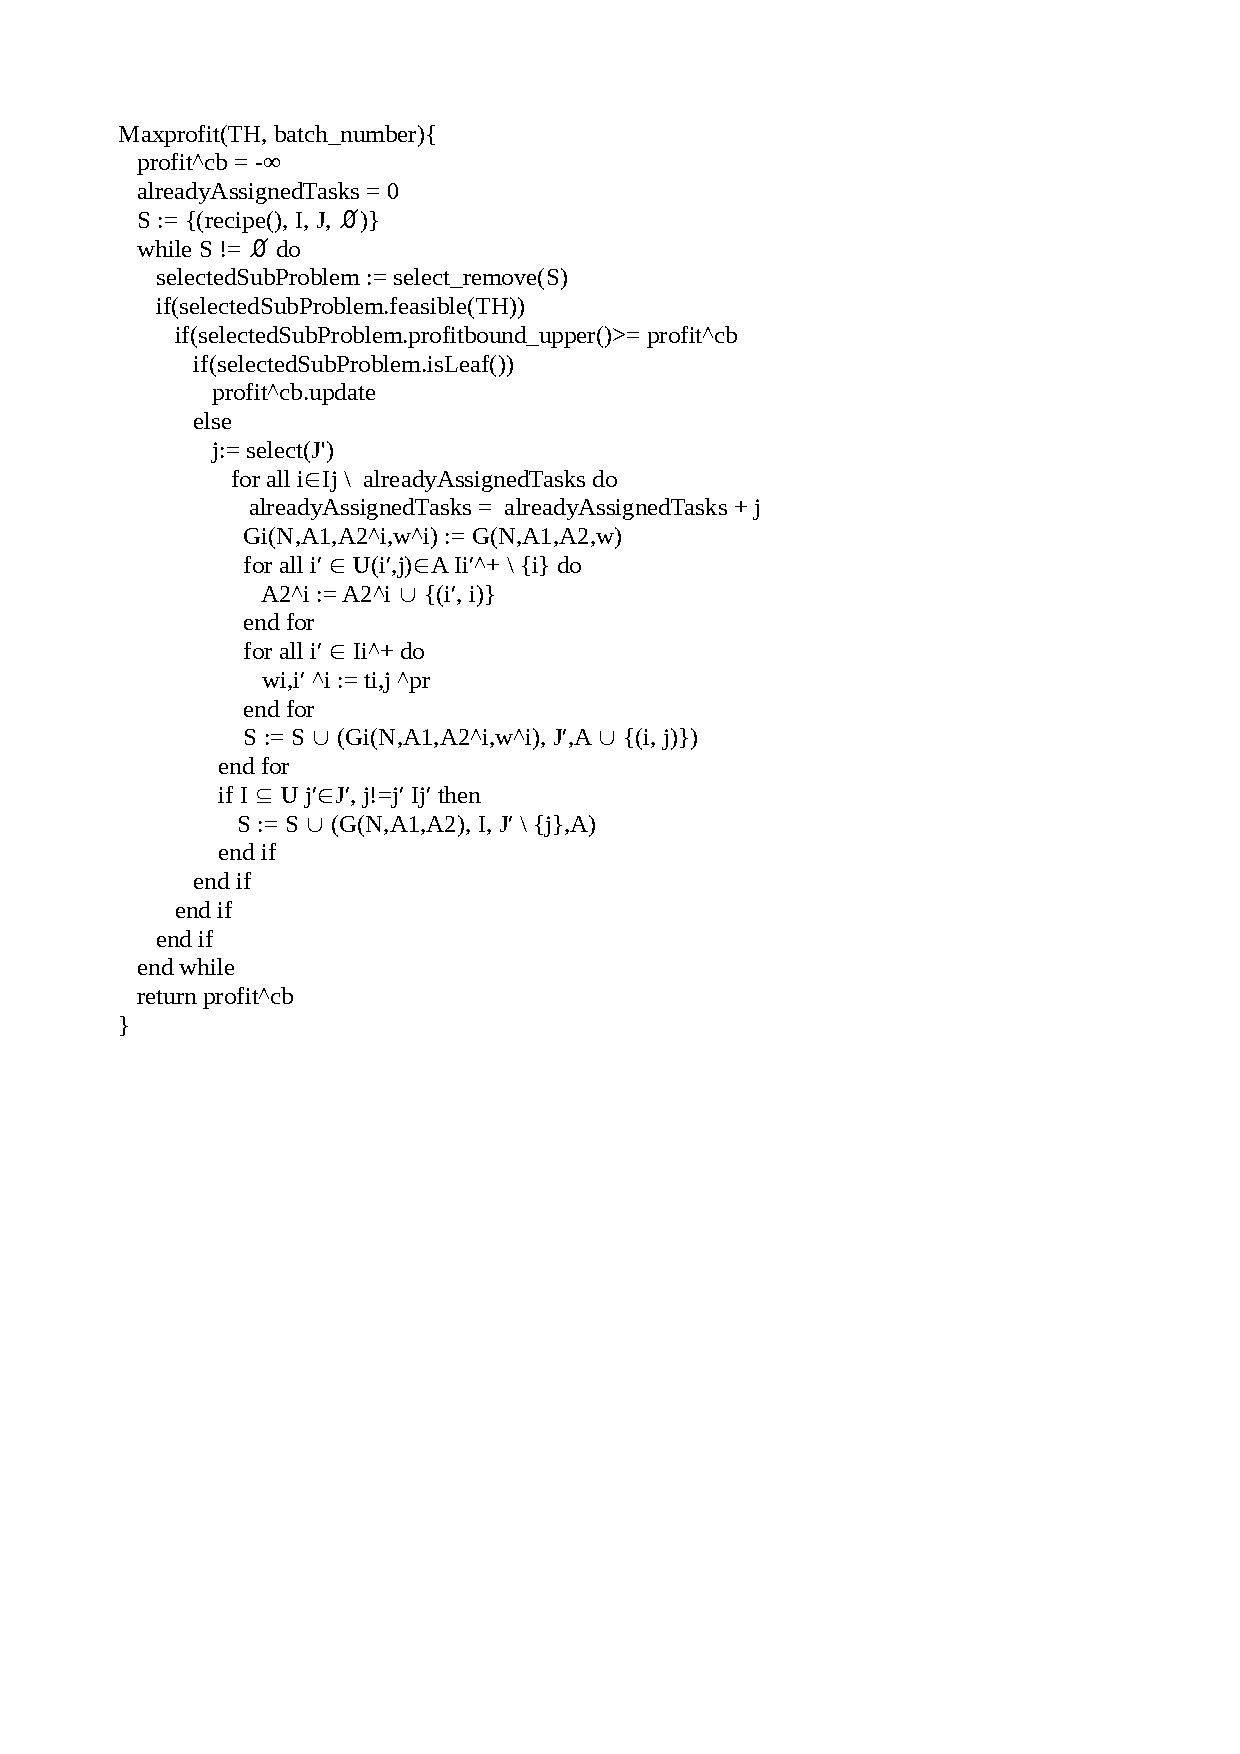
\includegraphics[scale=0.8]{uj_pszeudo}
%\caption{Pszeudó kód}
%\label{uj_pszeudo}
%\end{center}
%\end{figure}

\begin{algorithm}
\caption{Párhuzamos taszkvégrehajtást megvalósító algoritmus}
\begin{algorithmic}[1]
\Procedure{Maxprofit}{TH,batchsize}
	\State $profit^{cb} = -\infty$
	\State $SOAA:= \emptyset$
	\State $S:= {(recipe(),I,J,\emptyset)}$
	\While{$S \neq \emptyset$}
		\State $PP:= select\_remove(S)$
		\If {$PP.Feasible(TH)$}
			\If{$PP.proift\_bound > profit^{cb}$}
				\If{$PP.IsLeaf()$}
					\State $profit^{cb}.Update(PP.proift\_bound)$
				\Else
					\State $j:=select(J')$
					\ForAll	{$i \in I_j \setminus SOAA$}
						\State $SOAA^i: = SOAA^i\cup j$
						\State $G^i(N,A_1^i,A_2^i,w^i):= G(N,A_1,A_2,w)$
						\ForAll	{$i' \in \bigcup_{(i',j) \in \alpha} I_{i^i}^+  \setminus \{i\} $}
							\State $A_2^i:= A_2^i \cup \{(i',i)\}$				
						\EndFor
						\ForAll {$ i' \in I_i^+$}
							\State $w_{i,i'}^i:= t_{i,j}^{pr}$
						\EndFor
						\State $S:= S \cup (G^i(N,A_1,A_2^i,w^i),J',\alpha \cup \{(i,j)\})$
					\EndFor
					\If{$I \subseteq \bigcup_{SOAA^i = \emptyset, j = j'}I_j' $}
						\State $S:= S \cup (G(N,A_1,A_2),J'\setminus\{j\},\alpha)$
					\EndIf
				\EndIf
			\EndIf
		\EndIf
	\EndWhile
	\State \Return $profit^{cb}$
\EndProcedure
\end{algorithmic}
\end{algorithm}